\documentclass[usenames,dvipsnames,9pt]{beamer}
\usetheme[block=fill]{ru}           % Use ru theme

\usepackage{xpatch}
\usepackage{listings}
\usepackage{realboxes}

\definecolor{mygray}{rgb}{0.9,0.9,0.9}
\lstset{%
basicstyle=\ttfamily,
breaklines = true,
backgroundcolor=\color{mygray},
}

\makeatletter
\xpretocmd\lstinline{\Colorbox{mygray}\bgroup\appto\lst@DeInit{\egroup}}{}{}
\makeatother

\title{Advance Use of Git}

\author[Viguier]
{Beno\^{i}t Viguier}

\date[Short Occasion]{\vspace{0.5cm}DS-Lunch Talk,\\Nijmegen, October 25th, 2019}

\begin{document}

% -------------------------------------------------------------

% -------------------------------------------------------------
\begin{frame}
  \titlepage
\end{frame}

% -------------------------------------------------------------

% -------------------------------------------------------------
\begin{frame}{Disclaimer}
\begin{center}
  \alert{\Large{\textbf{If you don't line command line interface,\\this talk is not for you.}}}
\end{center}
\end{frame}


\begin{frame}{Git}

\end{frame}

\begin{frame}{Minimal Git Commands}
  \begin{itemize}
    \item \lstinline|git clone git@gitlab.science.ru.nl:user/repo|
    \item \lstinline|git status|
    \item \lstinline|git add <directory/files>|
    \item \lstinline|git commit|
    \item \lstinline|git push|
    \item \lstinline|git pull|
  \end{itemize}
\end{frame}



%%%%%%%%%%%%%%%%%%%%%%%%%%%%%%%%%%%%%%%%%%%%%%%%%%%%%%%
%
%           Git Status
%           Git Log
%
%%%%%%%%%%%%%%%%%%%%%%%%%%%%%%%%%%%%%%%%%%%%%%%%%%%%%%%
\begin{frame}{Git Status}
\begin{itemize}
  \item \lstinline|git status|
  \item \lstinline|git log|
\end{itemize}

\includegraphics[width=0.8\textwidth]{img/inspecting/01.png}
\end{frame}


\begin{frame}{Shortcuts}
\begin{itemize}
  \item \lstinline|git add --all| \hspace{1cm}(\lstinline|-A|)\\
  \emph{Add all the updated/untracked files.}
  \item \lstinline|git add --update| \hspace{1cm}(\lstinline|-u|)\\
  \emph{Add all the updated files but do not add the untracked ones.}
  % \item \lstinline|git commit -a|\\
  % \emph{Equivalent to:} \lstinline|git add -u ; git commit|
  \item \lstinline|git commit -m "commit message"|
\end{itemize}
\end{frame}



\section{branches}

%%%%%%%%%%%%%%%%%%%%%%%%%%%%%%%%%%%%%%%%%%%%%%%%%%%%%%%
%
%          Branches
%
%%%%%%%%%%%%%%%%%%%%%%%%%%%%%%%%%%%%%%%%%%%%%%%%%%%%%%%
\begin{frame}{Branches}
\begin{itemize}
  \item Develop features without breaking master.\\
  $\implies$ the master branch always compiles! {\color{OliveGreen}\checkmark}
  \item Develop multiple features at the same time.

\end{itemize}
\vspace{0.5cm}
\includegraphics[width=0.8\textwidth]{img/branches/01.png}
\end{frame}

\begin{frame}{Branches}
  \vspace{-0.45cm}
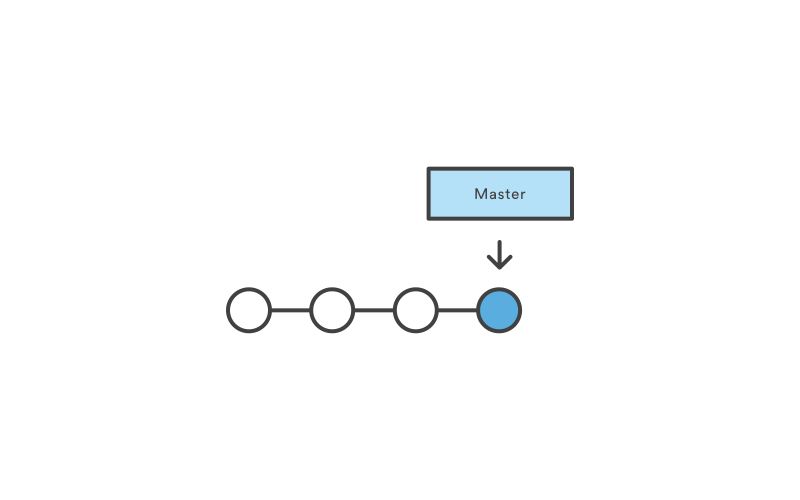
\includegraphics[width=0.8\textwidth]{img/branches/02.png}
\end{frame}

\begin{frame}{Branches}
  \begin{itemize}
    \item Create a branch \lstinline|git branch Future-plans|
    \item Switch to that branch \lstinline|git checkout Future-plans|
  \end{itemize}
\vspace{-1cm}
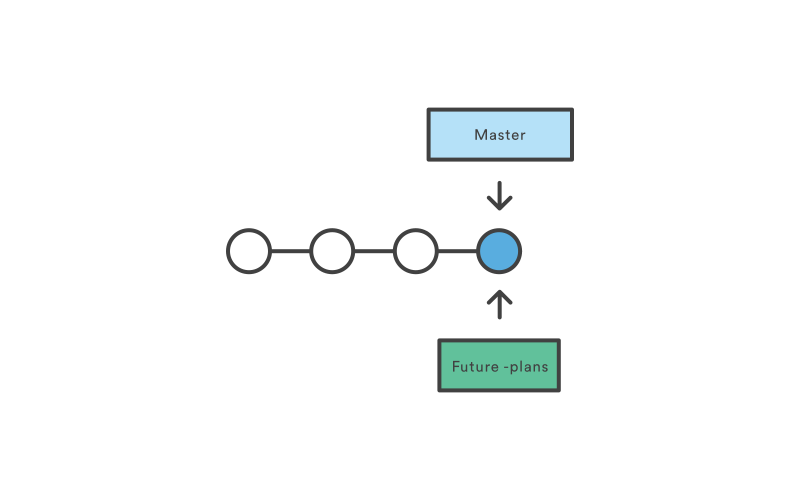
\includegraphics[width=0.8\textwidth]{img/branches/03.png}
\vspace{-1cm}

These two can be done in one step: \lstinline|git checkout -b Future-plans|
\end{frame}

\begin{frame}{Branches}
Work (modify, commits\ldots) on the \texttt{Future-plans}.\\
In the mean time, the \texttt{Master} branch continue forward (other commits\ldots)
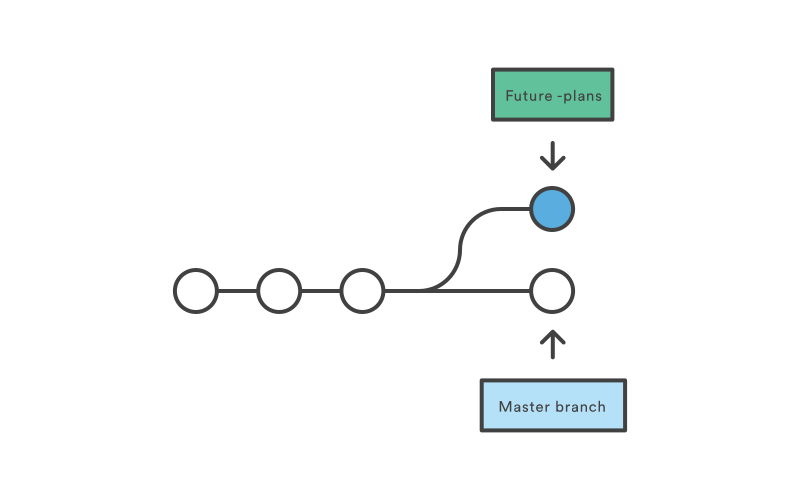
\includegraphics[width=0.8\textwidth]{img/branches/04.png}
\end{frame}


\begin{frame}{Branches}
If nothing was done on \texttt{Master} while you were working on \texttt{Future-plans} you can directly merge. This is called \emph{fast-forward}.
\begin{enumerate}
  \item Switch to the master branch: \lstinline|git checkout master|
  \item Merge: \lstinline|git merge Future-plans|
\end{enumerate}
\vspace{-1cm}
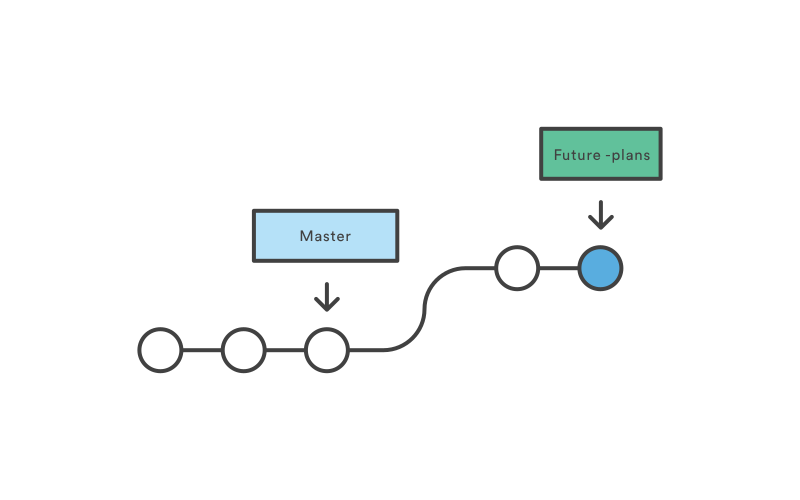
\includegraphics[width=0.8\textwidth]{img/branches/05.png}
\end{frame}

\begin{frame}{Branches}
\vspace{0.2cm}
If nothing was done on \texttt{Master} while you were working on \texttt{Future-plans} you can directly merge. This is called \emph{fast-forward}.
\begin{enumerate}
  \item Switch to the master branch: \lstinline|git checkout master|
  \item Merge: \lstinline|git merge Future-plans|
\end{enumerate}
\vspace{-0.8cm}
\hspace{0.07cm}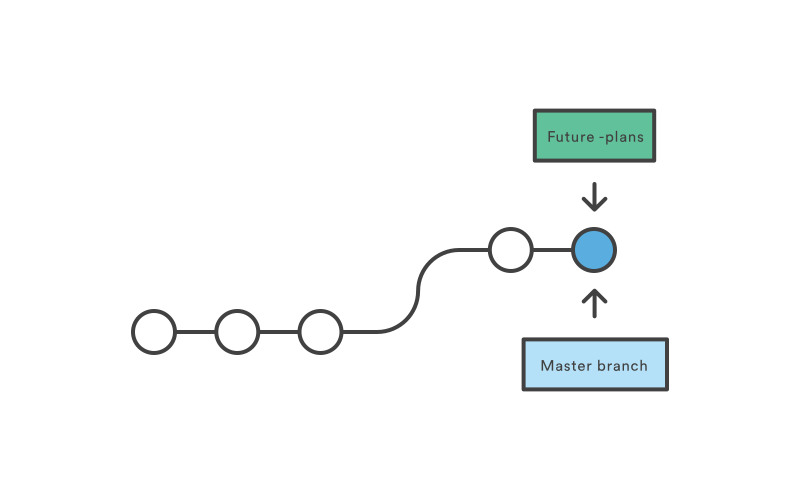
\includegraphics[width=0.8\textwidth]{img/branches/06.png}
\end{frame}

\begin{frame}{Branches}
  \centering
  To push/update a branch on the online repository:\\
  \lstinline|git push origin Future-plans|\\
  \vspace{1cm}
  To delete (\lstinline|-d|) a branch on the online repository:\\
  \lstinline|git push -d origin Future-plans|\\
  \vspace{1cm}
  To delete (\lstinline|-D|) locally a branch:\\
  \lstinline|git branch -D <branch-name>|\\
  (Not possible while you are on that branch.)
\end{frame}



\section{Merging}

%%%%%%%%%%%%%%%%%%%%%%%%%%%%%%%%%%%%%%%%%%%%%%%%%%%%%%%
%
%          Merging
%
%%%%%%%%%%%%%%%%%%%%%%%%%%%%%%%%%%%%%%%%%%%%%%%%%%%%%%%

\begin{frame}{Merging}
\texttt{Master} has changed while you were working on \texttt{Future-plans} the merge process is slightly different.
\begin{enumerate}
  \item Switch to the master branch: \lstinline|git checkout master|
  \item Merge: \lstinline|git merge Future-plans|
  \item Edit the commit message in your editor, save and close.
\end{enumerate}
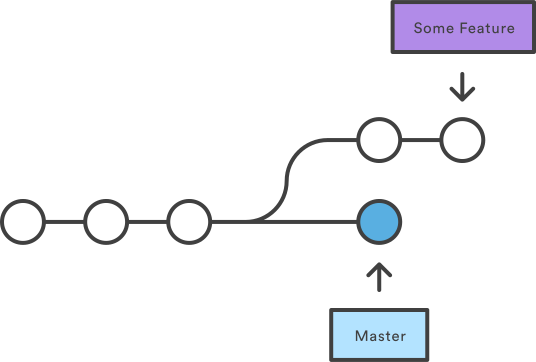
\includegraphics[width=0.608\textwidth]{img/merge/08.png}
\end{frame}

\begin{frame}{Merging}
  \texttt{Master} has changed while you were working on \texttt{Future-plans} the merge process is slightly different.
  \begin{enumerate}
    \item Switch to the master branch: \lstinline|git checkout master|
    \item Merge: \lstinline|git merge Future-plans|
    \item Edit the commit message in your editor, save and close.
  \end{enumerate}
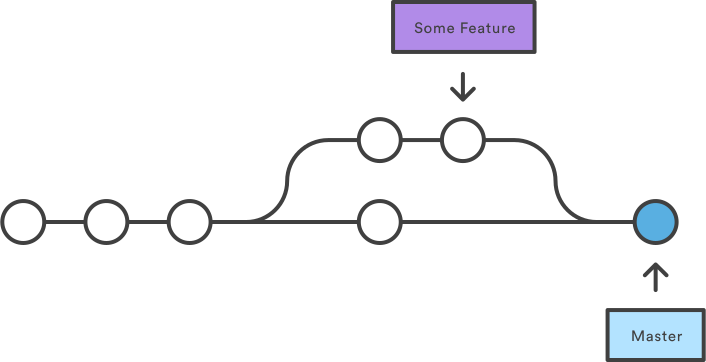
\includegraphics[width=0.8\textwidth]{img/merge/09.png}
\end{frame}

%%%%%%%%%%%%%%%%%%%%%%%%%%%%%%%%%%%%%%%%%%%%%%%%%%%%%%%
%
%          Rebase
%
%%%%%%%%%%%%%%%%%%%%%%%%%%%%%%%%%%%%%%%%%%%%%%%%%%%%%%%

\section{Rebasing}

\begin{frame}{Merging \& Rebasing}
\texttt{Master} has changed while you were working on \texttt{Feature}.\\
You want to make sure your modification do not break \texttt{Master}.\\
\vspace{0.37cm}
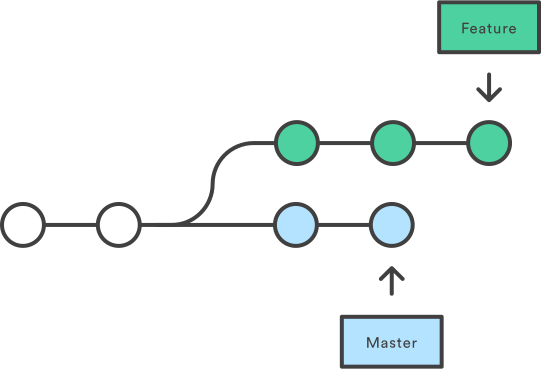
\includegraphics[width=0.59\textwidth]{img/merge/01.png}
\end{frame}

\begin{frame}{Merging}
Solution 1:
\begin{enumerate}
  \item Switch to the master branch: \lstinline|git checkout Feature|
  \item Merge: \lstinline|git merge Master|
\end{enumerate}
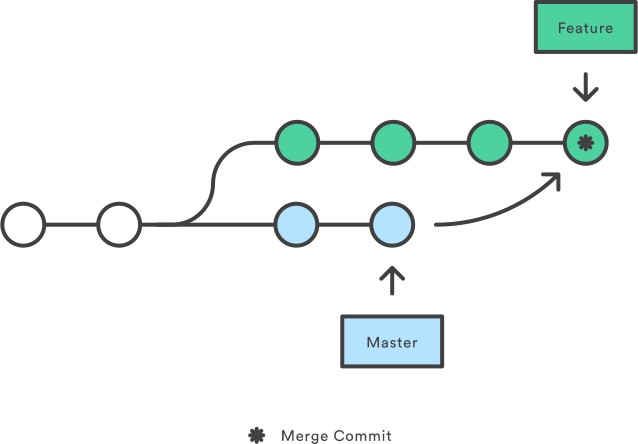
\includegraphics[width=0.695\textwidth]{img/merge/02.png}
\end{frame}

\begin{frame}{Rebasing}
Solution 2:
\begin{enumerate}
  \item Switch to the master branch: \lstinline|git checkout Feature|
  \item Merge: \lstinline|git rebase Master|
\end{enumerate}
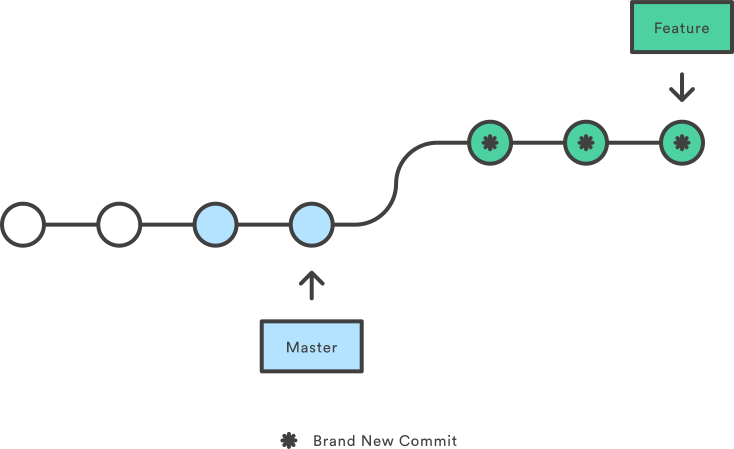
\includegraphics[width=0.8\textwidth]{img/merge/03.png}
\vspace{-0.06cm}
\end{frame}


\begin{frame}{Changing the commit message}
  You can rewrite the message of the last commit with:\\
  \lstinline|git commit --amend|

  \vspace{0.5cm}
  \includegraphics[width=0.5\textwidth]{img/rewriting/01.png}
\end{frame}
\begin{frame}{Changing the commit message}
  You can rewrite the message of the last commit with:\\
  \lstinline|git commit --amend|

  \vspace{0.5cm}
  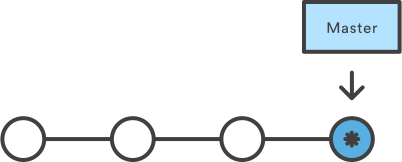
\includegraphics[width=0.5\textwidth]{img/rewriting/02.png}
\end{frame}

%%%%%%%%%%%%%%%%%%%%%%%%%%%%%%%%%%%%%%%%%%%%%%%%%%%%%%%
%
%          Reset
%
%%%%%%%%%%%%%%%%%%%%%%%%%%%%%%%%%%%%%%%%%%%%%%%%%%%%%%%

\section{HEAD, Checking out, Reverting \& Resetting}

\begin{frame}[t]{HEAD \& checkout}
\vspace{0.5cm}
The pointer of the current location in Git is called the \textbf{HEAD}.
It can be used as a reference point.

E.g. if you want to go back to a previous commit, you can do either:
\begin{itemize}
  \item \lstinline|git checkout HEAD~2|
  \item \lstinline|git checkout b|
\end{itemize}

\vspace{0.53cm}
\includegraphics[scale=1.5]{img/undoing/git-sequence-transparent.png}
\end{frame}

\begin{frame}[t]{HEAD \& checkout}
\vspace{0.5cm}
The pointer of the current location in Git is called the \textbf{HEAD}.
It can be used as a reference point.

E.g. if you want to go back to a previous commit, you can do either:
\begin{itemize}
  \item \lstinline|git checkout HEAD~2|
  \item \lstinline|git checkout b|
\end{itemize}

\vspace{0.5cm}
\includegraphics[scale=1.5]{img/undoing/2497537634-git-checkout-transparent.png}

From there you can start working on a new branch: \lstinline|git checkout -b Foo|
\end{frame}

\begin{frame}{Reverting}
If you want to undo the last commit: \lstinline|git revert HEAD|\\
This will \textbf{create} a new commit which reverts the last changes.

\vspace{0.5cm}
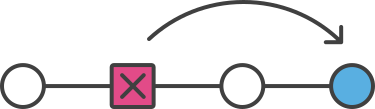
\includegraphics[width=0.5\textwidth]{img/undoing/02.png}

If you want to undo the change of an older commit you can also do:
\lstinline|git revert commit_id| e.g. \lstinline|git revert a1e8bf5|

\end{frame}

\begin{frame}{Resetting}
\lstinline|git reset --... commit_id| comes with 2 main options:
\begin{itemize}
  \item \lstinline|--soft|: keep the files as but reset the pointer to \lstinline|commit_id|.
  \item \lstinline|--hard|: reset the files to the pointer \lstinline|commit_id|.
\end{itemize}

\vspace{0.5cm}
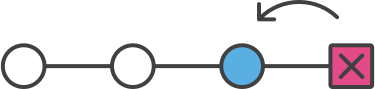
\includegraphics[width=0.5\textwidth]{img/undoing/03.png}

\end{frame}

\begin{frame}{Reset tricks}

\begin{itemize}
  \item \lstinline|git reset --hard HEAD|: remove all the change made from the HEAD\\~\\
  \item \lstinline|git reset --soft HEAD~4|: go back and forget 4 commits but leave the files as is. Usefull if you want to squash your history.\\~\\
  \item \lstinline|git reset --hard commit_id|: set the repository as it was in \lstinline|commit_id|
\end{itemize}

\end{frame}



%%%%%%%%%%%%%%%%%%%%%%%%%%%%%%%%%%%%%%%%%%%%%%%%%%%%%%%
%
%          Bonus
%
%%%%%%%%%%%%%%%%%%%%%%%%%%%%%%%%%%%%%%%%%%%%%%%%%%%%%%%

\section{Bonus}


\begin{frame}[fragile]{bonus}
  In your \texttt{~\char`\\.bashrc} or \texttt{~\char`\\.zshrc}:

  \texttt{alias gtree='git log --oneline --decorate --all --graph'}
\end{frame}
% commit
% branch
% checkout
% cherry-pick
% reset
% revert
% rebase
% merge
% cherry-pick



% <<<<<<< HEAD
% =======
% >>>>>>> new_branch_to_merge_later



\end{document}
